\chapter{Related Works}
\label{chap:relatedWorks}
This chapter presents the basic concepts  of indoor positioning systems the most widely used technologies and gives a brief overview of the mathematical background of modeling and filtering  time series.
\section{Indoor Positioning}
The first Indoor positioning systems were planned in the 1980s but they become popular in the last decade \cite{liu2007survey,gu2009survey}. 
IPS systems can be used in hospitals, malls, airports and offices.
Indoor positioning is challenging due to the unique properties of the indoor environment.
GPS is a very popular method of position, however it is not suited for such tasks because of its line of sight requirements and the multi path effect.
Wireless LAN, Bluetooth, infrared, ultrasonic and radio frequency  technologies are the most popular.
Active Badge \cite{want1992active} was the first indoor positioning system which was based on infrared signals.
Fingerprinting methods were first presented by the RADAR system \cite{bahl2000radar}.
RFID \cite{ni2004landmarc} based technologies has emerged in the last years.
Hybrid Indoor Positioning Systems \cite{baniukevic2013hybrid} has been created in the least few years.
This paper connects to the ILONA System which is a hybrid indoor positioning and navigation framework. \cite{ZsoltToth2015}.


\subsection{Indoor Positioning with Wireless LAN}
	Wireless LAN(WLAN) was designed to transmit data wirelessly over small distances, and connecting to the internet. WLAN also can be used for indoor positioning purposes \cite{evennou2006advanced}. WLAN is highly available since most devices can receive and process WLAN signals, smart phones can be programmed easily so they can implement client side filtering methods. It is also very cost-effective since the data received is highly accurate in most situations. Received Signal Strength Indication is measured by the device and it is determined for each available Access Points.
	 WLAN positioning is based on the measurement of the signal strength value (RSSI). The user  is linked to or multiple Access Points(AP) to determine user location at any given time. The User has to have a relatively stable and continuous connection. Unfortunately, the RSSI signal is not stable. It fluctuates over time even without any environmental impact. This fluctuation can be filtered at client side Electromagnetic signals are reflected \cite{kjaergaard2012mobile} by most bodies, as it can be seen on Figure \ref{fig:kockahaz}.
	\begin{figure}[h]
		\centering
		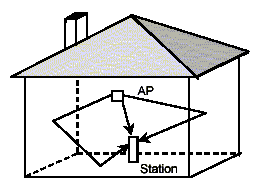
\includegraphics[width=.3\linewidth]{figures/Reflect.png}
		\caption{Indoor WLAN signal reflection \cite{Reflections}}\label{fig:kockahaz}
	\end{figure}
	 A few people in a room can drastically alter the measurements, making it less reliable the more reflective bodies there are in the room. 

\subsection{Fingerprinting Methods}
	Although WLAN was not developed to be a positioning system, it is a popular candidate for indoor positioning systems.  Most of the existing solutions are based on the fingerprinting technique \cite{kaemarungsi2004properties,honkavirta2009comparative}. Instead of determining the distance between the AP and the user by the  RSSI, it creates a radio map. Fingerprinting based indoor positioning methods require huge computational capacity, so they can be performed only on the server side.
	
\subsection{WiFi Based Solutions}
WiFi \cite{chen2002signal} based positioning popular due to the spread of mobile and smart phones in the early 2000's. However, GPS and AGPS are available in the modern phones, these technologies cannot be used in indoor environment. As more buildings, like hospitals, malls, etc. are designed with indoor WiFi Access Points in mind, it is only natural to try and use these APs to determine location.
\subsection{Horus System}
The Horus \cite{youssef2005horus} system is location determining system based on the IEE 802.11b WiFi , and Bluetooth connection, as seen on \ref{fig:horusimage}. The system determines user location by the received RSSI values from the access points. RSSI values are sent automatically, so implementing the system is purely a software solution, requiring no modifications on the hardware.
\begin{figure}[!h]
	\centering
		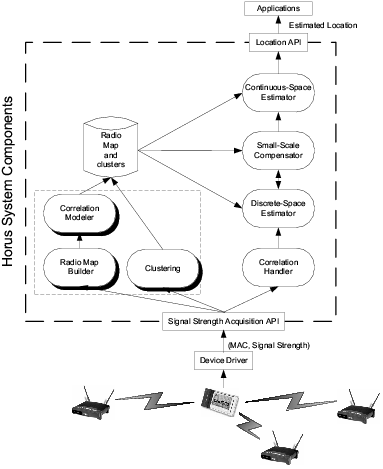
\includegraphics[width=.55\linewidth]{figures/Horus.png}
		\caption{Horus System \cite{HORUS}}\label{fig:horusimage}
\end{figure}


\section{Time Series Filtering Methods}
\subsection{Time Series}
Time series \cite{kalman1960new,durbin2012time} is a set of observations (x), being recorded a specified time (t).
It is stochastic in a sense that most of the time, measurements closer together have more importance towards each other.
Time series are often plotted with line charts on a one dimensional panel, as they represent the data fluctuations well.
They are very frequently used in most domain of applied science.

\subsection{Discrete Time Series}
A discrete time series is one which the set $T_0$ of times at which observations are made is a discrete set, for example being recorded at fixed time intervals. It is called continuous, if the measurements are being recorded continuously over a set amount of time.
\subsection{ARMA Models}
The three main modelling variations of importance are the autoregressive(AR),
moving average (MA), and the integrated (I) models. The ARMA modelling of wifi rssi will be the topic of a future research.


AR(p) refers to the autoregressive model of order p
$$ 
X_t = c + \sum_{i=1}^p \varphi_i X_{t-i}+ \varepsilon_t .\, 
$$
where $\varphi_1, \ldots, \varphi_p$ are parameters, c is a constant, and the random variable $\varepsilon_t$ is white noise.

Some constraints are necessary on the values of the parameters so that the model remains stationary. For example, processes in the AR(1) model with $|\phi_1| \geq 1$ are not stationary.

The notation MA(q) refers to the moving average model of order q:
$$
X_t = \mu + \varepsilon_t + \sum_{i=1}^q \theta_i \varepsilon_{t-i}\,
$$
where the $\theta_1, ..., \theta_q$ are the parameters of the model, $\mu$ is the expectation of $X_t$ (often assumed to equal 0), and the$ \varepsilon_t, \varepsilon_{t-1},...$ are again, white noise error terms.


The notation ARMA(p, q) refers to the model with p autoregressive terms and q moving-average terms. This model contains the AR(p) and MA(q) models,
$$
X_t = c + \varepsilon_t + \sum_{i=1}^p \varphi_i X_{t-i} + \sum_{i=1}^q \theta_i \varepsilon_{t-i}.\,
$$
The general ARMA model was described in the 1951 thesis of Peter Whittle, who used mathematical analysis (Laurent series and Fourier analysis) and statistical inference.


\subsection{Filtering Methods}
Filtering is the method of separating the noise from the signal, prediction of future values and control of current and future values.


\subsection{Time Windowing}
Time windowing is the process of allowing certain methods to stay idle for a certain amount of time before continuing to run or terminate. This certain amount of time depends on the predefined amount, and can be modified in the code. It is purely a software solution on most cases. Programs cannot andvence without any imput. Introducing a time window can make the program dynamic, because it can respond if it doesn't receive the needed values.
